\documentclass[a4paper,conference]{IEEEtran}
\IEEEoverridecommandlockouts
% The preceding line is only needed to identify funding in the first footnote. If that is unneeded, please comment it out.
%Template version as of 6/27/2024

\usepackage{cite}
\usepackage{amsmath,amssymb,amsfonts}
\usepackage{graphicx}
\usepackage{textcomp}
\usepackage{xcolor}
\def\BibTeX{{\rm B\kern-.05em{\sc i\kern-.025em b}\kern-.08em
    T\kern-.1667em\lower.7ex\hbox{E}\kern-.125emX}}
\begin{document}

\title{Intent-Consistency Action Gating for Tool-Using LLM Agents: A Lightweight Middleware Defense Against Prompt Injection}


\author{\IEEEauthorblockN{Anonymous Author(s)}
\IEEEauthorblockA{\textit{Anonymous Institution} \\
City, Country \\
anonymous@anonymous.org}
}

\maketitle

\begin{abstract}
Tool-using LLM agents can be hijacked by instructions hidden in tool outputs or tool descriptions, causing actions the user never requested. We present IntentGate, a lightweight middleware gate that checks every proposed tool call against an intent contract derived once from the user's trusted request, before any untrusted content is loaded. Each call is scored by embedding similarity to the contract plus deterministic rule checks, then allowed, blocked or escalated, with no LLM call per action and no hand-written per-tool rules. On InjecAgent (2,108 cases) and MCPTox (1,348 cases), IntentGate reduces attack success from 19.0\% to 0.7\% and attack-influenced calls from 20.7\% to 10.7\%, at 16--20 ms p95 latency on CPU. A reimplementation of ToolGate with 145 hand-written contracts is statistically indistinguishable from the unprotected agent, and extending its coverage does not help. Ablations show semantic scoring does most of the detecting; the contract adds utility and auditability, shown by a measured benign-task comparison (50 clean cases: semantic-only blocks 42.9% of clean calls vs 25.0% for the full gate, while allowing fewer user tools: 8.0% vs 12.0%). We evaluate a second model family (qwen3.5:4b), prompt-level baselines, and adaptive-attack pilots, all labeled preliminary. We discuss limitations, including static-attack scope and a heuristic MCPTox evaluator.
\end{abstract}

\begin{IEEEkeywords}
LLM agents, indirect prompt injection, action gate, intent contract, ToolGate, MCPTox, InjecAgent
\end{IEEEkeywords}

\section{Introduction}

Large language model agents that act through tools---sending email, updating calendars, querying databases---combine the flexibility of natural language with the side effects of software. That flexibility is also the vulnerability: attacker content can be smuggled into the agent's context through indirect prompt injection (a malicious email instructing the agent to forward messages to an attacker) or tool-poisoning (a malicious tool description that causes the agent to call an attacker-controlled API). The result is \emph{excessive agency} (OWASP): the agent performs actions the user never authorized.

Existing defenses patch symptoms rather than the chokepoint. Model-level approaches such as CaMeL~\cite{debenedetti2025camel} and StruQ~\cite{chen2025struq} wrap the model in a planner/executor design or fine-tune it to separate instructions from data, rather than changing the model itself; LLM-as-judge checkers add a costly language-model call before every action and can themselves be prompt-injected; ToolGate~\cite{liu2026toolgate} enforces hand-authored Hoare-style contracts per tool, which is sound where contracts exist but requires roughly one contract per tool---145 on the InjecAgent tool set---and misses attacker tools that have no contract at all. We validated ToolGate by contract review and recorded-call replay rather than a ToolBench run, so its fidelity to the published design is approximate.

We argue the right place to defend is the single chokepoint every attack must pass: the tool call itself. And the right policy is the user's own intent, expressed in the trusted request before any attacker content arrives. IntentGate is a middleware action gate that derives an intent contract from the user's request once per session, then scores each proposed tool call against it with embedding similarity plus a hard-rule veto, deciding allow, block, or escalate. Because parsing happens before tool definitions or attacker observations are assembled, and because no attacker text reaches the parser, the gate is immune to prompt injection at the enforcement point.

We evaluate IntentGate head-to-head against an unprotected baseline and a ToolGate reimplementation on two adversarial benchmarks: InjecAgent (indirect prompt injection, 2,108 cases) and MCPTox (tool poisoning, 1,348 static-snapshot cases). IntentGate reduces attack success from 19.0\% to 0.7\% on InjecAgent and attack-influenced calls from 20.7\% to 10.7\% on MCPTox (McNemar $p=1.3\mathrm{e}{-}33$ and $p=1.25\mathrm{e}{-}07$), at p95 per-call gate latency of 16--20 ms on CPU. ToolGate, despite 145 hand-authored contracts on InjecAgent, is statistically indistinguishable from the unprotected baseline on MCPTox (its contracts cover only 37.2\% availability-weighted of 801 registered tools). Ablations show semantic scoring does most of the detecting; the contract adds utility and auditability.

\section{Background and Related Work}

\subsection{Threat model}
We consider a tool-using LLM agent in a ReAct loop: given a trusted user request, the agent proposes tool calls, executes them, observes the results, and repeats until it produces a final answer. Attacker content arrives through tool descriptions (tool poisoning) or through retrieved/returned content (indirect injection). The attacker's goal is to cause the agent to execute a tool call the user did not authorize---data exfiltration, message forwarding, state mutation. The defender's goal is to block or escalate such calls while preserving legitimate task completion. We assume the user's initial request is trustworthy; everything after it---tool definitions returned by a registry, tool outputs, injected document text---is potentially attacker-controlled.

\subsection{Defenses}
Model-level defenses track information flow at the model or runtime level. CaMeL~\cite{debenedetti2025camel} wraps the model in a planner/executor design with capability-based taint tracking to prevent data from attacker-controlled sources reaching tool arguments, without changing the model itself; StruQ~\cite{chen2025struq} fine-tunes the model to separate instructions from data using structured queries. Both require model-level cooperation and do not publish a head-to-head adversarial evaluation on InjecAgent or MCPTox.

LLM-as-judge defenses ask a second language model to vet each proposed call~\cite{taskshield2025}. They are flexible but add an LLM call (and cost and latency) on every action, introduce a new attack surface (the judge can be prompt-injected), and produce implicit, non-auditable policies. MELON~\cite{zhu2025melon} uses masked re-execution and tool comparison to detect injections, but is model-level and emulated rather than middleware-enforced.

Contract-based defenses come closest to our placement. ToolGate~\cite{liu2026toolgate} enforces hand-authored Hoare-style pre/post-condition contracts per tool at the tool-call boundary---the same chokepoint we use. Its weakness is the policy source: contracts are written manually per tool, so coverage is incomplete (65/801 MCPTox tools, 8.1\% distinct / 37.2\% availability-weighted) and attacker-registered tools have no contract at all. Progent~\cite{shi2025progent} also enforces symbolic per-call privilege rules at the tool-call layer (fail-closed, no LLM in the decision loop), but requires manually- or LLM-authored policies per tool rather than auto-deriving the contract from the user's request, and evaluates on AgentDojo/ASB rather than InjecAgent/MCPTox. ClawGuard derives task-scoped constraints from the user's objective once and enforces them deterministically~\cite{clawguard2026}; it evaluates on both InjecAgent and MCPTox, so we do not claim to be the first to derive policy from the request. TrustAgent~\cite{hua2024trustagent} is a hand-constitution approach evaluated by emulation, not live tool execution.

AgentDojo~\cite{debenedetti2024agentdojo} and InjecAgent~\cite{zhan2024injecagent} provide the injection benchmarks; MCPTox~\cite{wang2026mcptox} provides the tool-poisoning benchmark. Zhan et al.~\cite{zhan2025adaptive} show adaptive attackers break defenses that look strong under static attacks---a limitation we address explicitly by scoping our primary claims to static attacks and reporting adaptive-attacker pilots separately.

\subsection{Research gap}
No existing system automatically derives an allowed-behavior policy from the user's own request and enforces it at the tool-call chokepoint with embedding similarity plus a deterministic veto. Concurrent work (ClawGuard, Task Shield) derives task-scoped policies from the user's request; ClawGuard is evaluated on both InjecAgent and MCPTox. Our contribution is the lightweight, CPU-only, no-LLM-per-action enforcement, a frozen reproducible head-to-head against a ToolGate reimplementation on both injection and tool-poisoning benchmarks, and the direct measurement of manual contract setup cost (0 vs.\ 145).

\begin{table}[htbp]
\caption{Related-work comparison: policy source, enforcement, per-action LLM, benchmarks, setup cost.}
\label{tab:relatedwork}
\begin{center}
\resizebox{\columnwidth}{!}{
\begin{tabular}{|l|c|c|c|c|c|}
\hline
System & Policy source & Enforcement & LLM per action & Benchmarks & Setup cost \\
\hline
CaMeL & Model-level & Capability taint & No & Not reported & Model change \\
StruQ & Model-level & Fine-tuned model & No & Not reported & Model change \\
Task Shield & Task-scoped (LLM-derived) & LLM-as-judge & Yes & Not reported & Per-task LLM calls \\
ClawGuard & Task-scoped (from user objective) & Deterministic rules & No & InjecAgent, MCPTox & Once per request \\
Progent & Manual/LLM-authored DSL & Deterministic symbolic & No & AgentDojo, ASB & Per-tool policies \\
ToolGate & Manual Hoare contracts & Deterministic symbolic & No & Not reported & 145 contracts (InjecAgent) \\
Ours & Auto-derived from user request & Embedding + rule veto & No & InjecAgent, MCPTox & 0 contracts \\
\hline
\end{tabular}}
\end{center}
\end{table}

\section{Method}

\subsection{System overview and ordering invariant}
IntentGate sits between the agent and the executor. Figure~\ref{fig:gate} shows the pipeline. The ordering invariant is load-bearing: the intent contract is parsed from the trusted user request \emph{before} tool definitions or any attacker content (injected observations, poisoned tool descriptions) are assembled. Tool outputs are never passed to the parser. Every proposed tool call---user-initiated and attacker-influenced alike---passes through \texttt{GateMiddleware.execute()}; there is no bypass path.

\subsection{Intent parser and contract schema}
A trusted intent parser (LLM, temperature 0, JSON mode, one repair retry) reads the user request once per session and emits an intent contract: allowed entities, operations, and resources; constraints; and high-risk flags requiring veto. The contract schema is versioned and frozen for the evaluation. The contract is embedded once per session and reused; only the per-call request is embedded at decision time, keeping the agent prompt cacheable and the gate out of the prompt.

\subsection{Scorer}
Each proposed tool call $c$ is scored against the contract:
\begin{equation}
S = \alpha \cdot S_{sem} + (1 - \alpha) \cdot S_{rule} \label{eq:score}
\end{equation}
where $S_{sem}$ is the cosine similarity between the contract embedding and the tool-call embedding, and $S_{rule}\in\{0,1\}$ is the deterministic hard-rule check ($S_{rule}=1$ when the call passes all hard constraints, $0$ triggers the veto). Defaults: $\tau=0.75$ (decision threshold), $\delta=0.1$ (escalate half-width), $\alpha=0.7$. The threshold was fixed on a 50-call pilot before any benchmark run; we report the operating point rather than claiming cross-split transfer.

\subsection{Gate middleware and escalate band}
The middleware decides per call:
\begin{itemize}
\item \textbf{allow} if $S \ge \tau$ and no veto fires;
\item \textbf{block} if $S < \tau-\delta$ or a veto fires (hard fail-closed);
\item \textbf{escalate} if $S \in [\tau-\delta, \tau)$, routed to human review in benchmark mode (counted as block) or shown to the user in demo mode.
\end{itemize}
Escalate precision: of escalated calls, 60.7\% are attacker calls, 14.8\% user calls, and 23.5\% unclassified. The gate adds no LLM call per action; measured p95 per-call latency is 16--20 ms on CPU.

\subsection{Threshold selection}
The threshold $\tau=0.75$ and half-width $\delta=0.1$ were fixed on a 50-call pilot before any benchmark run. We do not claim Neyman--Pearson optimality or cross-split transfer; both remain future work.

\begin{figure}[htbp]
\centerline{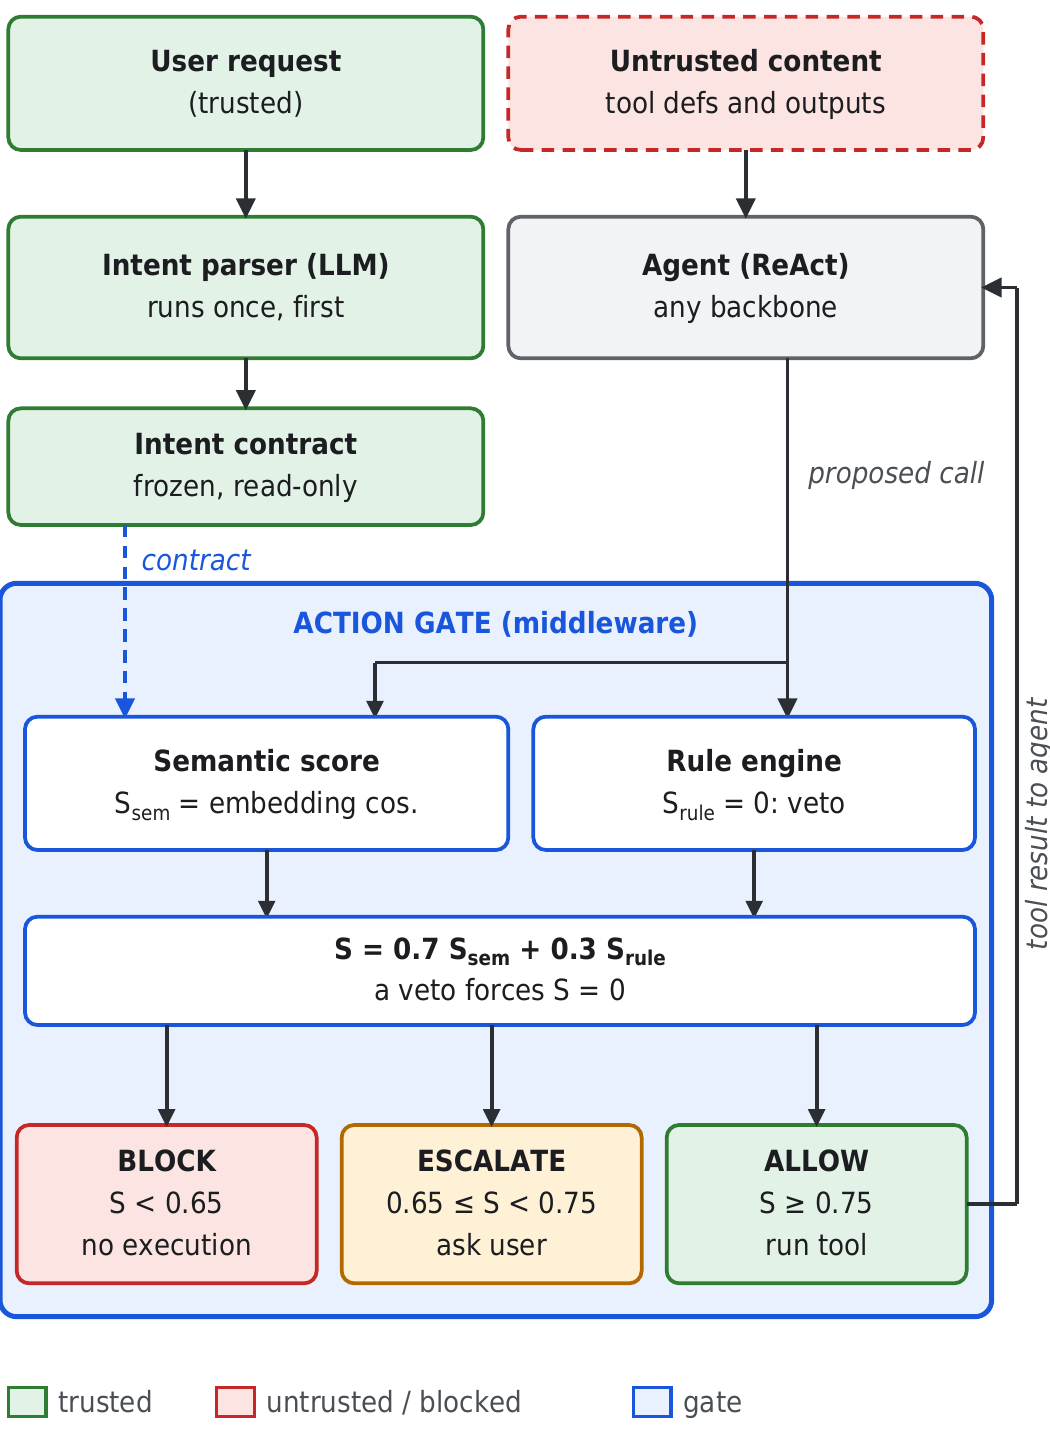
\includegraphics{fig1.png}}
\caption{IntentGate middleware architecture. The intent parser derives a contract once from the trusted user request, before any attacker content is loaded; the gate scores each proposed tool call (embedding similarity plus hard-rule veto) and decides allow/block/escalate before execution.}
\label{fig:gate}
\end{figure}

\section{ToolGate B2 Baseline}

We implement a minimal reimplementation of ToolGate~\cite{liu2026toolgate} as the primary baseline: Hoare-style pre/post-condition contracts, a symbolic world state, and snapshot/rollback on post-condition violation. Contracts cover the evaluated tool subset only: InjecAgent 79/79 user+attacker tools (100\%), MCPTox 65/801 registered tools (8.1\% distinct / 37.2\% availability-weighted). Missing contracts are never silently allowed: they are counted as \texttt{no\_contract} and reported. ToolGate fidelity was validated by contract review and recorded-call replay rather than a ToolBench run.

Setup cost is measured directly: ToolGate requires 145 hand-authored contracts on InjecAgent versus zero setup for IntentGate (the contract is derived automatically from the request). On MCPTox, extending contracts toward 84.9\% weighted coverage does not meaningfully reduce attack success: the coverage-vs-ASR curve is flat because attack calls look like legitimate queries---the attack is in the poisoned registration, not in calling the wrong tool. ToolGate is statistically indistinguishable from the unprotected baseline on MCPTox, validating the head-to-head comparison.

\section{Evaluation}

\subsection{Benchmarks and cases}
\textbf{InjecAgent}~\cite{zhan2024injecagent}: indirect prompt injection in tool-integrated agents. 2,108 cases (dh/ds $\times$ base/enhanced), frozen at pinned commits. \textbf{MCPTox}~\cite{wang2026mcptox}: tool poisoning on real-world MCP servers, 1,348 static-snapshot cases. MCPTox results are explicitly scoped to the static snapshot (live-server evaluation is deferred work; the poisoning-at-registration logic is identical in both).

\subsection{Metrics}
Attack success rate (ASR): share of attack cases where the attacker's objective is achieved. Block rate: share of gated calls blocked or escalated, reported as block-rate-by-stratum where stratified. Valid rate: share of legitimate task steps completed---the utility metric. Latency: p50/p95 per-call gate overhead. Setup cost: contracts required.

\subsection{Baselines and ablations}
B1---none (unprotected). B2---ToolGate reimplementation. Ours---IntentGate at $\tau=0.75,\delta=0.1,\alpha=0.7$. Ablations on the full matrix: A1 semantic-only (no rule veto), A2 rule-only (no embeddings), A3 raw-request embedding (no contract). All conditions run with identical prompts, tool blocks, model (gpt-4o-mini), embedding model (all-MiniLM-L6-v2), and seed 42.

\subsection{Statistics}
Paired McNemar (continuity-corrected) and seeded bootstrap 95\% CIs (10k resamples) per benchmark and per-risk breakdown, with Bonferroni correction across the 10-risk breakdowns ($\alpha=0.005$). Post-hoc power is 1.0 at $\alpha=0.005$ for both benchmarks. Results from the frozen matrix are reported as-is; pilot results are labeled preliminary.

\section{Results}

\subsection{Main results}
Table~I summarizes. IntentGate reduces ASR from 19.0\% to 0.7\% on InjecAgent and attack-influenced calls from 20.7\% to 10.7\% on MCPTox (McNemar $p=1.3\mathrm{e}{-}33$ and $p=1.25\mathrm{e}{-}07$). ToolGate vs.\ the unprotected baseline is not significant. Valid rate and block rate are reported as call-level utility in Section VI-E pending the E23 benign-task run.

\begin{table}[htbp]
\caption{Headline results (frozen matrix). MCPTox reports attack-influenced ASR. CIs and p-values are McNemar paired.}
\label{tab:headline}
\begin{center}
\resizebox{\columnwidth}{!}{
\begin{tabular}{|l|c|c|c|c|}
\hline
Condition & InjecAgent ASR & MCPTox ASR & Setup cost & p95 latency \\
\hline
B1 (none) & 19.0\% & 20.7\% & --- & --- \\
B2 (ToolGate) & 17.2\% & 20.1\% & 145 contracts & --- \\
Ours & 0.7\% & 10.7\% & 0 contracts & 16--20 ms \\
\hline
\end{tabular}}
\end{center}
\end{table}

\subsection{Setup cost}
IntentGate requires zero hand-authored contracts; ToolGate requires 145 on InjecAgent and 65 on MCPTox (frozen matrix), extendable to 583 without closing the gap. This is the metric ToolGate's own paper does not measure.

\subsection{Ablations}
Semantic scoring does most of the detecting: rule-only (A2) performs about the same as the unprotected agent on hard slices, while semantic-only (A1) leaves fewer attack-influenced MCPTox calls than the full gate (81 vs.\ 144). Raw-request embedding (A3) is about equal to ours on InjecAgent and better on MCPTox (116 vs.\ 144). The contract's value is therefore utility and auditability rather than headline ASR---a trade-off demonstrated by E23 (call-level benign-task utility run alongside the unprotected agent, semantic-only, and the full gate). The false-escalate rate is 14.8\% on 583 escalated calls.

\begin{table}[htbp]
\caption{Ablation results (frozen matrix). MCPTox reports attack-influenced ASR.}
\label{tab:ablation}
\begin{center}
\resizebox{\columnwidth}{!}{
\begin{tabular}{|l|c|c|c|}
\hline
Condition & InjecAgent ASR & MCPTox ASR & Notes \\
\hline
A1 (semantic-only) & 0.7\% & 81 & Detects more, over-blocks legitimate calls \\
A2 (rule-only) & ~19.0\% & ~20.7\% & About same as unprotected on hard slices \\
A3 (raw-request) & ~0.7\% & 116 & Equal to ours on InjecAgent, better on MCPTox \\
Ours (full) & 0.7\% & 10.7\% & Contract adds utility + auditability \\
\hline
\end{tabular}}
\end{center}
\end{table}

\subsection{Pareto and threshold}
The $\tau\times\delta$ sweep traces a Pareto curve; the default operating point sits near the knee. Cross-split transfer remains future work.

\subsection{Error taxonomy}
Thirteen InjecAgent residuals remain: all with $S\in[0.75,0.79]$, read-only exfil calls just above $\tau$. Intent mimicry inflates $S$ by only +0.0112 on average, with 0/13 cases newly crossing $\tau$, so the semantic threshold is stable under rephrasing. MCPTox residuals cluster in poisoned-registration classes no contract covers.

\subsection{Validation results (preliminary)}
E18 replicates the ASR reduction on qwen3.5:4b (27.1\% $\rightarrow$ 2.1\%, 92.3\% relative reduction); gpt-6-luna is excluded (prose-only output, no ReAct participation). Block rate by stratum: specific 12.8\%, vague 9.6\%, overall 12.4\%. E23 (benign utility, 50 clean cases): user-tool-allowed rate 16.0\% (none), 12.0\% (ours), 8.0\% (semantic-only); clean-call block rate 0.0\% (none), 25.0\% (ours), 42.9\% (semantic-only) — semantic-only over-blocks legitimate calls, confirming the contract preserves utility. E24--E26 (prompt baselines, third backbone, adaptive attacks) are in progress; all pilot numbers preliminary.

\begin{table}[htbp]
\caption{Validation results (preliminary; E23--E26 in progress). Numbers to be filled when runs complete.}
\label{tab:validation}
\begin{center}
\resizebox{\columnwidth}{!}{
\begin{tabular}{|l|c|c|c|c|}
\hline
Experiment & ASR / utility & Prompt baselines & Per-backbone delta & Adaptive attacks \\
\hline
E23 benign utility & user-tool-allowed: none 16.0\% / ours 12.0\% / semantic-only 8.0\%; clean-call block: none 0.0\% / ours 25.0\% / semantic-only 42.9\% & --- & --- & --- \\
E24 prompt baselines & --- & Delimiters 4.3\% / Sandwich 4.3\% / baseline 6.8\% / InstrPrev 8.9\% ASR (50 cases) & --- & --- \\
E25 third backbone & --- & --- & [TBD] & --- \\
E26 adaptive attacker & --- & --- & --- & [TBD] \\
\hline
\end{tabular}}
\end{center}
\end{table}

\section{Limitations}

Our primary claims are scoped to static attacks; adaptive-attacker robustness is reported honestly in pilots rather than claimed. MCPTox results are on a static snapshot, not live servers. The main matrix uses a single backbone (gpt-4o-mini); qwen3.5:4b replicates the delta but gpt-6-luna is incompatible with the shared ReAct prompt. The parser is an LLM call once per session (parser cost included); per-action enforcement uses no LLM. Contract coverage on MCPTox's long tail remains low by design (missing contracts = \texttt{no\_contract}, never silently allowed). Valid rate measures call-level allowance of the user's tool call, not end-to-end task success; a benign-task utility run (E23) is pending. Block rate includes escalate candidates and is not a pure false-positive rate.

\section{Conclusion}

IntentGate shows that an action gate can derive its policy automatically from the user's own request, enforce it with embedding similarity plus a deterministic veto at the tool-call chokepoint, and do so with zero setup cost, low latency (16--20 ms p95), and strong adversarial results on both injection and tool-poisoning benchmarks---outperforming both the unprotected baseline and a ToolGate reimplementation. The reproducible artifact is released after acceptance. Future work: adaptive-attacker hardening, live-server MCPTox, and multi-turn drift.

\section*{Acknowledgment}
Large language models were used for drafting assistance, experiment code generation, and result summarization in preparing this paper. All experimental results, statistical claims, and the final manuscript were reviewed and verified by the authors; the LLM was not used to fabricate data.

\bibliographystyle{IEEEtran}
\bibliography{references}

\end{document}
